%%%%%%%%%%%%%%%%%%%%
%%%%%%%%%%%%%%%%%%%%
%%
%% Andrea Tino - 2019
%% Programming + Science
%% Opinion model
%%
%%%%%%%%%%%%%%%%%%%%
%%%%%%%%%%%%%%%%%%%%

\section{Developing a CA to describe people's opinion change}
\label{sec:opinionca}

In section \ref{sec:simpleca}, we have built our first automaton: Conway's Game of Life.
That CA is a great start because it has many interesting configurations and evolutions;
however, now, we want to move forward and develop another, different, automaton.
A CA is a mathematical model; other than being a very fun thing to play with, it is a
tool that can be used to study our reality from a theoretical perspective. Like any other
model, it is capable of simplifying our universe so that we can study specific things
about a natural phenomenon. CGL was just an automaton we built without a specific goal
in mind, we just wanted to play with automata.
For the next stage, we want to build a CA that can help us reach a distinct objective:
illustrating opinion change among the members of a society.

\subsection{Working out the model}
We want to use a scientific approach to solve a problem. So, 
before going straight to coding, we need to:

\begin{enumerate}
\item Decide what natural phenomenon we want to describe and control. 
We basically want to answer the question: what is the problem we want to solve?
\item Define the mathematical model to reach that objective. We 
basically need to translate
our problem into mathematical terms. This step is called: \textit{modelization}.
\item Create a computer simulation by translating into code the mathematical
model we created, this stage is called: \textit{simulation}. While simulating,
it is possible to collect all sorts of data and measurements; those will be used
to rate which model best achieves the objectives with highest performance and
lowest cost.
\item After all simulations have been run, the best model is selected and then
effectively put in practice. Most of the times, it results in something being
physically built, or a process being enforced. This stage is called:
\textit{implementation}.
\end{enumerate}

% Figure
%
\begin{figure}[b]
\centering
\sidecaption
% tikz diagram
%
% Tikz Diagram
%

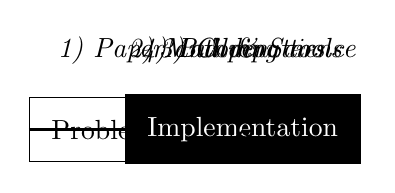
\begin{tikzpicture}

%\pgfdeclareimage{bulb}{assets/light-bulb}

\tikzmath{
	\x = 3.4;
    \sx = \x + \x;
    \ssx = \sx + \x;
    \y = -0.75;
}

\node[draw,inner sep=8pt] (prob) at (0,0) {Problem definition};
\node[draw,inner sep=8pt,fill=gray,text=white] (mod) at (\x,0) {Modelization};
\node[draw,inner sep=8pt,fill=black,text=white] (sim) at (\sx,0) {Simulation};
\node[draw,inner sep=8pt,fill=black,text=white] (impl) at (\ssx,0) {Implementation};

\draw[->,draw=black,thick] (prob) to (mod);
\draw[->,draw=black,thick] (mod) to (sim);
\draw[->,draw=black,thick] (sim) to (impl);

%\node {\pgfbox[center,bottom]{\pgfuseimage{bulb}}};

\node at (0, \y) {\textit{1) Paper and pen}};
\node at (\x, \y) {\textit{2) Math \& Science}};
\node at (\sx, \y) {\textit{3) Computers}};
\node at (\ssx, \y) {\textit{4) Building tools}};

\end{tikzpicture}

%
% If not, use
%\picplace{5cm}{2cm} % Give the correct figure height and width in cm
%
\caption{Illustration of the different phases in the scientific approach to solve a problem.
Each one of them is executed with different tools and require different skills.}
\label{fig:sciappr}
\end{figure}
%

This way of doing things (visualized in figure \ref{fig:sciappr})
is called: \textit{scientific approach} and is at the very core
of what scientists, mathematicians and engineers do every day. So let's start
with the first step: what problem do we want to solve?

\begin{proposition}[Problem definition]
\label{prop:opinionproblem}
We want to
\end{proposition}

fg
